\chapter{Control Hijacking}

Application software is computer software that performs a group of pre-defined functions or tasks. It can provide services locally or remotely, and its behavior is determined by the data/input being processed, the code being executed, and the environment in which it runs. 

Compromising the security properties, i.e. \textbf{Confidentiality}, \textbf{Integrity}, and \textbf{Availability}, is the goal of attackers. But how can they achieve this?

\section{Attack}
Control hijacking attacks are a class of attacks that hijack the control flow of an application. Since application code is loaded into memory, attackers may corrupt memory through techniques such as buffer overflows, integer overflows, and format string exploitation. Before diving into the details, we first look at several related concepts.

\subsection{Control Flow Graph}
Applications may invoke external commands to perform specific tasks. For example, \texttt{system(<string>)} executes a command specified in a string by calling \texttt{/bin/sh -c <string>}. Therefore, once users control the string content, they can inject arbitrary commands.

\begin{minipage}{0.5\textwidth}
It is helpful to understand the behavior of an application, i.e. its control flow. This describes the order in which code is executed or interpreted, and it can represent the functionality or behavior of a program to some extent. \\[3pt]
We can use a \textbf{Control Flow Graph (CFG)} to graphically represent the control flow of a program. It shows all possible paths that might be traversed during the execution of the program. \\[3pt]
A Control Flow Graph contains nodes, which are blocks of code without branches, connected by directed edges. A CFG should have an entry node and an exit node. A path is a sequence of nodes connected by edges. Note that not all paths are feasible.
\end{minipage}
\begin{minipage}{0.5\textwidth}
\begin{figure}[H]
  \centering
  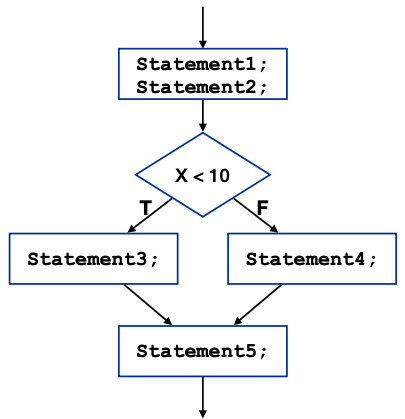
\includegraphics[width=0.6\textwidth]{Figure/CFG1.png}
  \caption{Control Flow Graph}
\end{figure}
\end{minipage}

\subsection{Program State}
A program state can be described by the values of processor registers and memory, such as the stack and heap.

Processor registers provide several quickly accessible storage locations. They hold data used in arithmetic and logical operations, and data is copied between registers and main memory as needed.

\begin{minipage}{0.5\textwidth}
For memory, the stack usually grows downward (toward lower memory addresses). The stack pointer \texttt{ESP} points to the top of the stack. The \texttt{push} instruction decrements \texttt{ESP} and stores a value at the address pointed to by \texttt{ESP}. The \texttt{pop} instruction retrieves the value at the top of the stack into a register and then increments \texttt{ESP}.\\[3pt]
The stack is composed of frames. Frames are pushed onto or popped from the stack when a function is invoked or returns. Each frame contains the function's actual parameters, the return address, a pointer to the previous frame, and the function's local variables (as shown in Figure~2.2). The stack base pointer \texttt{EBP} stores the address of the current frame.
\end{minipage}
\begin{minipage}{0.5\textwidth}
\begin{figure}[H]
  \centering
  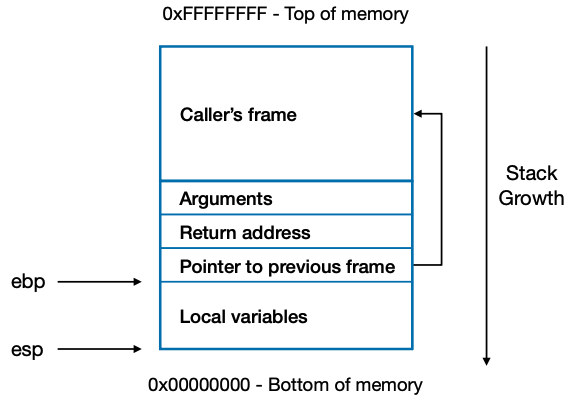
\includegraphics[width=0.9\textwidth]{Figure/StackFrame.png}
  \caption{Stack Frame Layout}
\end{figure}
\end{minipage}

A simple walkthrough of a function call can be illustrated using the following example:

\begin{minipage}{0.5\textwidth}
\begin{verbatim}
#include <ctype.h> // tolower
#include <string.h> // strcmp
#include <stdio.h> // fgets, fputs

void reveal_secret() {
  fputs("SUPER SECRET = 42\n", stdout);
}

int verify(const char* name) {
  char user[256];
  int i;
  for (i = 0; name[i] != '\0'; ++i)
    user[i] = tolower(name[i]);
  user[i] = '\0';
  return strcmp(user, "xyzzy") == 0;
}

int main() {
  char login[512];
  fgets(login, 512, stdin);
  if (! verify(login))
    return 1;
  reveal_secret();
  return 0;
}
\end{verbatim}
\end{minipage}
\begin{minipage}{0.5\textwidth}
\begin{figure}[H]
  \centering
  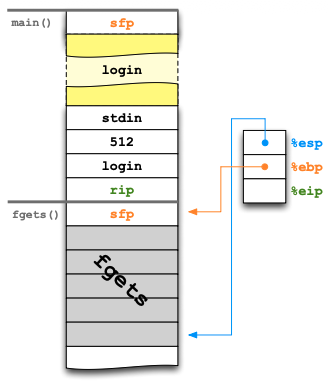
\includegraphics[width=0.9\textwidth]{Figure/FunctionCall.png}
  \caption{Stack - Function Call}
\end{figure}
\end{minipage}


Consider the entry point of this program at \texttt{int main()}. The saved frame pointer (SFP) points to the old frame pointer (OFP), which is pushed onto the stack, causing \texttt{ESP} to decrement. Since this is now the current frame, \texttt{EBP} will point to this position and will remain unchanged unless another function is called.

Next, \texttt{login[512]} is allocated on the stack. The program then reaches the first function call, \texttt{fgets}. The arguments of the function are pushed onto the stack in reverse order, i.e.\ \texttt{stdin}, \texttt{512}, and then \texttt{login}. After that, the return instruction pointer (RIP) is pushed onto the stack so that the program knows where to resume execution after the function call returns.

These steps repeat for subsequent function calls until the program finishes executing all function calls.

\subsection{Overflow}
Overflow is one of the most popular classes of attacks, as it is exploitable both locally and remotely, and it can modify both the data and the control flow of an application.

More specifically, we will discuss stack overflow. A function's local variables (buffers) are statically allocated on the stack, and data may be copied or written without boundary checking. Therefore, data can overflow a buffer and overwrite other important data, e.g.\ the return address or the saved \texttt{EBP}. With a carefully crafted input, it is possible to overwrite security-sensitive data, redirect execution to user-defined code, or even reuse existing code. We will examine three cases.

\begin{minipage}{0.4\textwidth}
\subsubsection{Overflow -- Crash}
Consider the example above. Suppose the user inputs a value of 500 bytes. After the \texttt{fgets} function call finishes, the program proceeds to the \texttt{verify(login)} function call. Inside \texttt{int verify}, the program iterates through the input and calls \texttt{tolower}. The resulting characters are then stored in the array \texttt{user[256]}.\\[3pt]
Since the length of \texttt{name} is 500, writing the data into \texttt{user[256]} causes the buffer to overflow. As a result, the content beyond \texttt{user[256]} overwrites other data on the stack, including the saved frame pointer and the return address (instruction pointer / program counter, \texttt{EIP}). When the function returns, the program attempts to jump to the corrupted return address. This typically redirects execution to an invalid or unknown address, causing the program to crash.
\end{minipage}
\begin{minipage}{0.6\textwidth}
\begin{figure}[H]
  \centering
  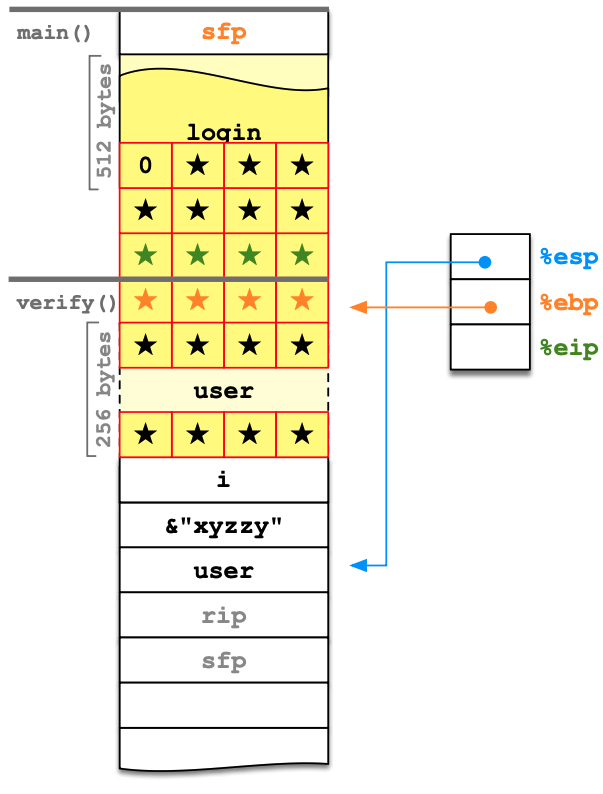
\includegraphics[width=0.7\textwidth]{Figure/FunctionCallCrash.png}
  \caption{Stack Overflow - Crash}
\end{figure}
\end{minipage}

\begin{minipage}{0.4\textwidth}
\subsubsection{Overflow -- Inject}
Assume the attacker provides input containing machine code (shellcode), e.g.

\begin{verbatim}
a0c2d782
ffa86db2
307abba9
ad7c....
\end{verbatim}

When this input is processed by the program (\texttt{user[i] = tolower(name[i])}), the bytes are copied into the buffer \texttt{user}. If the input exceeds the buffer size, a carefully crafted overflow can overwrite the saved frame pointer (SFP) and the saved return address (RIP). By replacing the saved return address with the address of the injected shellcode in the buffer, the attacker can cause the program to jump to the shellcode when the function returns. The shellcode can then execute a system call such as \texttt{execve("/bin/sh")} to spawn a shell.
\end{minipage}
\begin{minipage}{0.6\textwidth}
\begin{figure}[H]
  \centering
  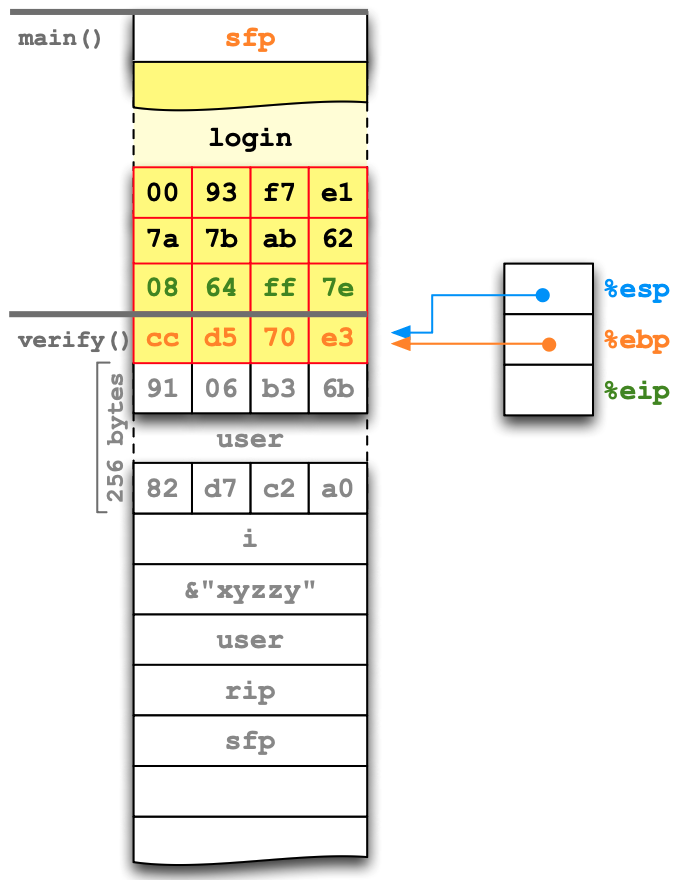
\includegraphics[width=0.7\textwidth]{Figure/FunctionCallInject.png}
  \caption{Stack Overflow - Inject}
\end{figure}
\end{minipage}

\begin{minipage}{0.4\textwidth}
\subsubsection{Overflow - Divert}
This type of overflow is similar to the code injection. Assume the address of \texttt{reveal\_secret} is \texttt{0xc8f4f2a9}. Similar to the previous case, with a carefully crafted overflow, the user can overwrite the return instruction pointer (RIP) with \texttt{0xc8f4f2a9}. Then, when the function call ends, the program will jump to \texttt{reveal\_secret} and display the message `SUPER SECRET \(=\) 42'.
\end{minipage}
\begin{minipage}{0.6\textwidth}
\begin{figure}[H]
  \centering
  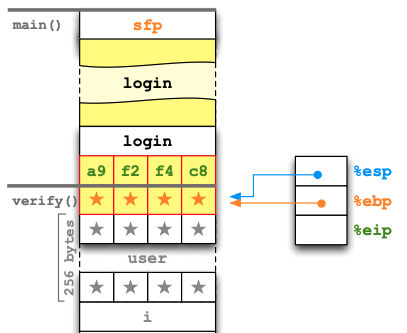
\includegraphics[width=0.7\textwidth]{Figure/FunctionCallDivert.png}
  \caption{Stack Overflow - Divert}
\end{figure}
\end{minipage}

There are several other vulnerable functions in C/C++, e.g.\ \texttt{fgets()}, \texttt{strcpy()}, \texttt{strcat()}, \texttt{sprintf()}, \texttt{vsprintf()}, \texttt{scanf()}, \texttt{sscanf()}, etc. Any reference to a value that can be overwritten may represent a security vulnerability. For example, we can overwrite the following:

1. Data and data pointers

2. Return address

3. Stack frame pointer

4. Exception handler

5. Function pointer

6. Jump destination

Therefore, safer versions of memory access functions should be used to ensure that important data structures, i.e.\ the stack, heap, and others, cannot be overwritten. However, there are still some possible overflows.

\textbf{Integer Overflow}

Integer overflow is caused by unexpected results when comparing, casting, or performing arithmetic operations on integers. There are several cases:

1. A large signed integer can become a negative value.

2. A large unsigned integer can become a small unsigned integer.

3. A negative signed integer can become a large unsigned integer.

Therefore, integers of different sizes or types should be assigned with great care, and assertions or similar checks can be used to avoid overflows.

\textbf{Index Overflow}

Index overflow exploits the lack of boundary checks when referencing a value in an array using an index. This allows direct writes to memory locations. Depending on the situation, it may only be possible to modify memory values that conform to the type of elements in the array.

For example, consider an array declared as \texttt{array[10]}. If the program reads input without checking the bounds and writes to a position beyond indices \(0\) to \(9\), it causes an overflow.

\begin{remark}
  In C++, objects can be dynamically allocated on the heap. Each object is associated with a pointer pointing to the virtual function table (vtable), which is a table of pointers to the definitions of the object's methods. A variable overflow can be used to overwrite this pointer so that it points to a fake virtual function table specified by the attacker.
\end{remark}